\section{Eulerian fluid simulation}

We have implemented the fluid simulation algorithm as described in the paper "Real-Time Fluid Dynamics for Games" by Jos Stam \cite{stable}.
This fluid is simulated using a velocity and density field.

\begin{figure}[h]
    \centering
    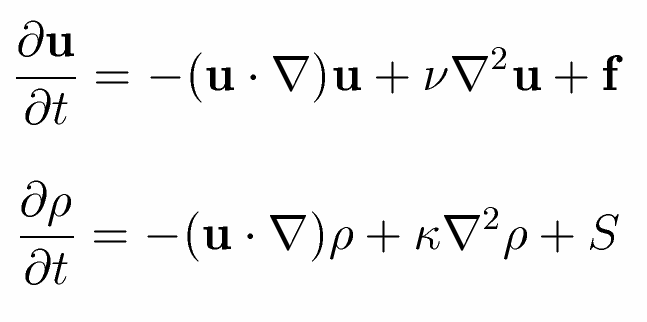
\includegraphics[width=5cm]{img/navierstokes.png}
    \caption{The Navier-Stokes Equations for the velocity in a compact vector notation (top) and the equation for a density moving through the velocity field (bottom).}
    \label{fig:navierstokes}
\end{figure}

\noindent The Navier-Stokes Equations are a precise description of the evolution of a velocity field over time.
Given the current state of the velocity and a forces, the equations tell us precisely how the velocity will change over an infinitesimal time step.
Figure~\ref{fig:navierstokes} (top) depicts these equations in a compact vector-like notation.
Very roughly the equation states that the change in velocity is due to the three terms on the right hand side of the equal sign.

\noindent The density usually takes values between zero and one: where there is no fluid the density is zero, and elsewhere it indicates the amount of particles present.
The evolution of the density field through the velocity field of the fluid can also be described by a precise mathematical equation,
which is depicted at the bottom of Figure~\ref{fig:navierstokes}.

\noindent We define a grid where both the density and velocity are defined at the cell centers.
The grid contains an extra layer of cells to account for the boundary conditions.

\subsection{Density}
The paper presents us with a solver for the velocity and density Navier-stokes equation at each time step.
For the density equation there are three terms on the right hand side of the equation.
The first term says that the density should follow the velocity field, the second states that the density may diffuse at a certain rate and the third term says that the density increases due to sources.

\noindent The fist step is solved by modeling the density as a set of particles.
Start with two grids: one that contains the density values from the previous time step and one that will contain the new values.
For each grid cell of the latter we trace the cell’s center position backwards through the velocity field.
We then linearly interpolate from the grid of previous density values and assign this value to the current grid cell.

\noindent The second step is solved by exchanging the density of each cell with its direct neighbors, as shown in Figure~\ref{fig:diffuse}.

\begin{figure}[h]
    \centering
    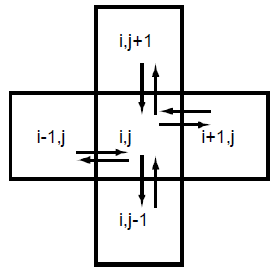
\includegraphics[width=4cm]{img/diffuse.png}
    \caption{Through diffusion each cell exchanges density with its direct neighbors.}
    \label{fig:diffuse}
\end{figure}

\noindent The density of a region is increased when the users selects it with the mouse.
Using diffusion and the velocity field this source automatically spreads.


\subsection{Velocity}
The velocity field uses the same advection step as the density field.
This is because the Navier-Stokes Equations are very similar.
The only extra addition to the velocity step is mass conservation.
This is an important property of real fluids which should be enforced.

\subsection{Boundry}
We assume that the fluid is contained in a box with solid walls: no flow should exit the walls.
This simply means that the horizontal component of the velocity should be zero on the vertical walls, while the vertical component of the velocity should be zero on the horizontal walls.
This is accomplished by inverting the velocity (w.r.t. x and y) on the boundaries and copying the density of its neighbours.
